\documentclass[border=8pt]{standalone}
\usepackage[utf8]{inputenc}
\usepackage{tikz}
\tikzset{
  entita/.style = {rectangle, draw, thick, fill=blue!8, minimum width=30mm, minimum height=20mm, font=\small},
  attr/.style   = {circle, draw, thick, fill=white, minimum size=5pt, inner sep=0},
  pk/.style     = {circle, draw, thick, fill=black, minimum size=5pt, inner sep=0},
  link/.style   = {thick}, et/.style = {font=\footnotesize}
}
\begin{document}
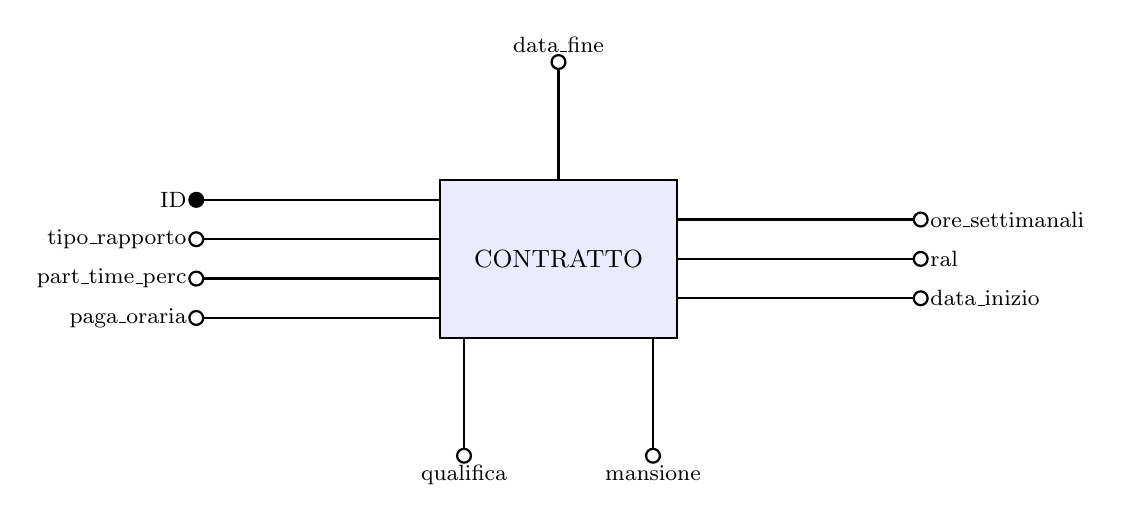
\begin{tikzpicture}
  \node[entita] (E) {CONTRATTO};

  % sinistra (4)
  \node[pk]   (id) at (-4.6, 0.75){}; \draw[link] (-1.5, 0.75)--(id); \node[et,left] at (id) {ID};
  \node[attr] (tr) at (-4.6, 0.25){}; \draw[link] (-1.5, 0.25)--(tr); \node[et,left] at (tr) {tipo\_rapporto};
  \node[attr] (pt) at (-4.6,-0.25){}; \draw[link] (-1.5,-0.25)--(pt); \node[et,left] at (pt) {part\_time\_perc};
  \node[attr] (po) at (-4.6,-0.75){}; \draw[link] (-1.5,-0.75)--(po); \node[et,left] at (po) {paga\_oraria};

  % destra (3)
  \node[attr] (os) at (4.6, 0.5){}; \draw[link] (1.5, 0.5)--(os); \node[et,right] at (os) {ore\_settimanali};
  \node[attr] (ral) at (4.6, 0.0){}; \draw[link] (1.5, 0.0)--(ral); \node[et,right] at (ral) {ral};
  \node[attr] (di)  at (4.6,-0.5){}; \draw[link] (1.5,-0.5)--(di);  \node[et,right] at (di)  {data\_inizio};

  % alto (1)
  \node[attr] (df) at (0,2.5){}; \draw[link] (0,1.0)--(df); \node[et,above] at (df) {data\_fine};

  % basso (2)
  \node[attr] (q) at (-1.2,-2.5){}; \draw[link] (-1.2,-1.0)--(q); \node[et,below] at (q) {qualifica};
  \node[attr] (m) at ( 1.2,-2.5){}; \draw[link] ( 1.2,-1.0)--(m); \node[et,below] at (m) {mansione};
\end{tikzpicture}
\end{document}
